\section{Tycho-2 Dataset}\label{sec:tycho-2Dataset}
\begin{figure}
    % https://www.cosmos.esa.int/web/gaia/iow_20150115
    \centering{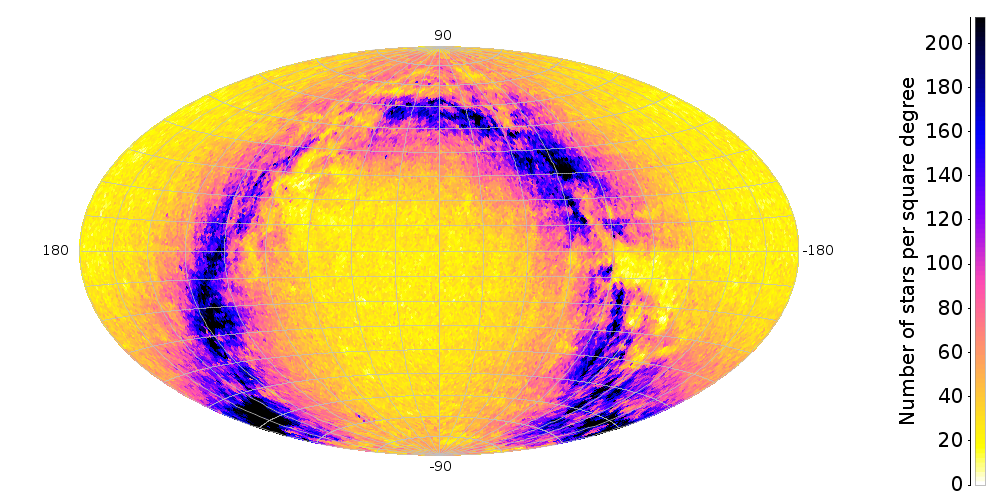
\includegraphics[scale=0.25]{images/tycho.png}}
    \caption{Heat map of the celestial sphere mapped by the Tycho-2 dataset.
    There exist roughly 2.5 million stars here.}\label{fig:tycho}
\end{figure}

In order to make decisions about our data model, we need to understand our data: a star catalog.
A star catalog is a collection of stars, their positions, and other traits, enumerated by their catalog numbers.
The Tycho-2 star catalog comes from the ESA (European Space Agency) astrometric mission Hipparcos, as well as other
existing catalogs.
This dataset is available at~\url{ftp://cdsarc.u-strasbg.fr/pub/cats/I/259}.

Typical star catalogs hold stars as points projected onto a 2D map of space known as the celestial sphere.
Each point is recorded as a vector ($\alpha, \delta$) in the \textit{Equatorial coordinate system}.
$\alpha$ represents right ascension, which is the celestial equivalent of longitude on Earth.
$\delta$ represents declination, which is the celestial equivalent of latitude.
~\autoref{fig:tycho} depicts a heat map of the stars inside the catalog, and is meant to illustrate how positions of stars are recorded.

There exist two main sections of interest here: the catalog files, and the index file.
The catalog files hold each star (or astronomical object), their astrometric properties, and their 3-number \texttt{TYC}
ID\@.
This is formatted as such:
\begin{alignat*}{3}
    &\texttt{TYC1} &&\texttt{TYC2} &&\texttt{TYC3} \\
    &\text{[Region \#]} \ \ \ \ &&\text{[Running \#]} \ \ \ \ &&\text{[Component Identifier]}
\end{alignat*}

Each \texttt{TYC1}, or \textit{GSC Region Number} corresponds to a specific region in space.
Region here, refers to a section on the celestial sphere.
Every GSC Region corresponds to, at most, a $3.75^\circ \times 3.75^\circ$ region of the sky.
The running number corresponds to a star inside that region, and the component identifier indicates how many stars
exist in that specific system (typically equal to 1).

Also contained are the proper motions of each star, the epoch (time) associated with the current record, the apparent
magnitude (brightness), and errors associated with all of the former.
For the queries tested here only the apparent magnitude, the $(\alpha, \delta)$, and the \texttt{TYC} IDs were recorded
with each entry.

The index file is sorted by \texttt{TYC1}, and holds the bounds representing each region $\left(\alpha_{min},
\alpha_{max}\right), \left(\delta_{min}, \delta_{max}\right)$.
Regions were recorded with each boundary and the appropriate \texttt{TYC1} ID\@.

%To simplify our problem, we define \textit{nearby} as sharing the same \texttt{TYC1} region.